\section{Introduction}
\label{sec:intro}
\IEEEPARstart{F}{reshwater} ecosystems, inland water bodies, transboundary river networks, natural wetlands, and artificial storage reservoirs sustain terrestrial biodiversity, global agricultural irrigation, municipal drinking supplies, and industrial activity~\cite{pekel2016high,rahimzadegan2021surface}. Over the past two decades, accelerating climate change, rapid demographic expansion, urban encroachment into vulnerable floodplains, and extreme hydro-meteorological shocks have exerted unprecedented strain on planetary water systems~\cite{taravat2021satellite}. Surface water bodies exhibit profound spatial and temporal variability, ranging from gradual seasonal shoreline shrinkage in arid endorheic basins to rapid, catastrophic flood inundation triggered by intense cloudbursts, tropical cyclones, atmospheric rivers, and dam breach crises~\cite{clement2018multi,boudjit2021sen12flood}. In emergency disaster response operations, rapid, high-resolution, and accurate mapping of standing water, inundated infrastructure, and river overflows is vital for guiding life-saving humanitarian logistics, civil defense evacuations, and post-disaster structural damage appraisal~\cite{brown2022dynamic}.

According to international disaster databases (e.g., CRED EM-DAT and UN-SPIDER reports), hydrological disasters account for over $44\%$ of all natural disasters worldwide, causing tens of thousands of fatalities and exceeding $\$50$ billion in annual direct economic losses. Achieving the United Nations Sustainable Development Goal 6 (Target 6.6: Protect and restore water-related ecosystems) and Goal 13 (Climate Action) requires continuous, high-frequency, and synoptic monitoring of surface water extent, volume variations, and inundation dynamics across transboundary river basins.

Traditional in situ hydrological monitoring techniques---including terrestrial streamflow gauging stations, river stage loggers, bathymetric sonar surveys, and manned airborne reconnaissance---are severely constrained by sparse geographic distribution, prohibitive capital and operational maintenance costs, data latency, and physical vulnerability during extreme weather events. In developing nations and remote transboundary wilderness regions, streamflow gauge networks are increasingly decommissioned due to budgetary constraints. Consequently, spaceborne satellite Earth Observation (EO) represents the only viable technology capable of providing synoptic, continuous, repeatable, and high-frequency surveillance of global surface water dynamics across transboundary river basins and remote wilderness areas~\cite{helber2018eurosat,hong2021spectralformer}.

\begin{figure*}[t]
\centering
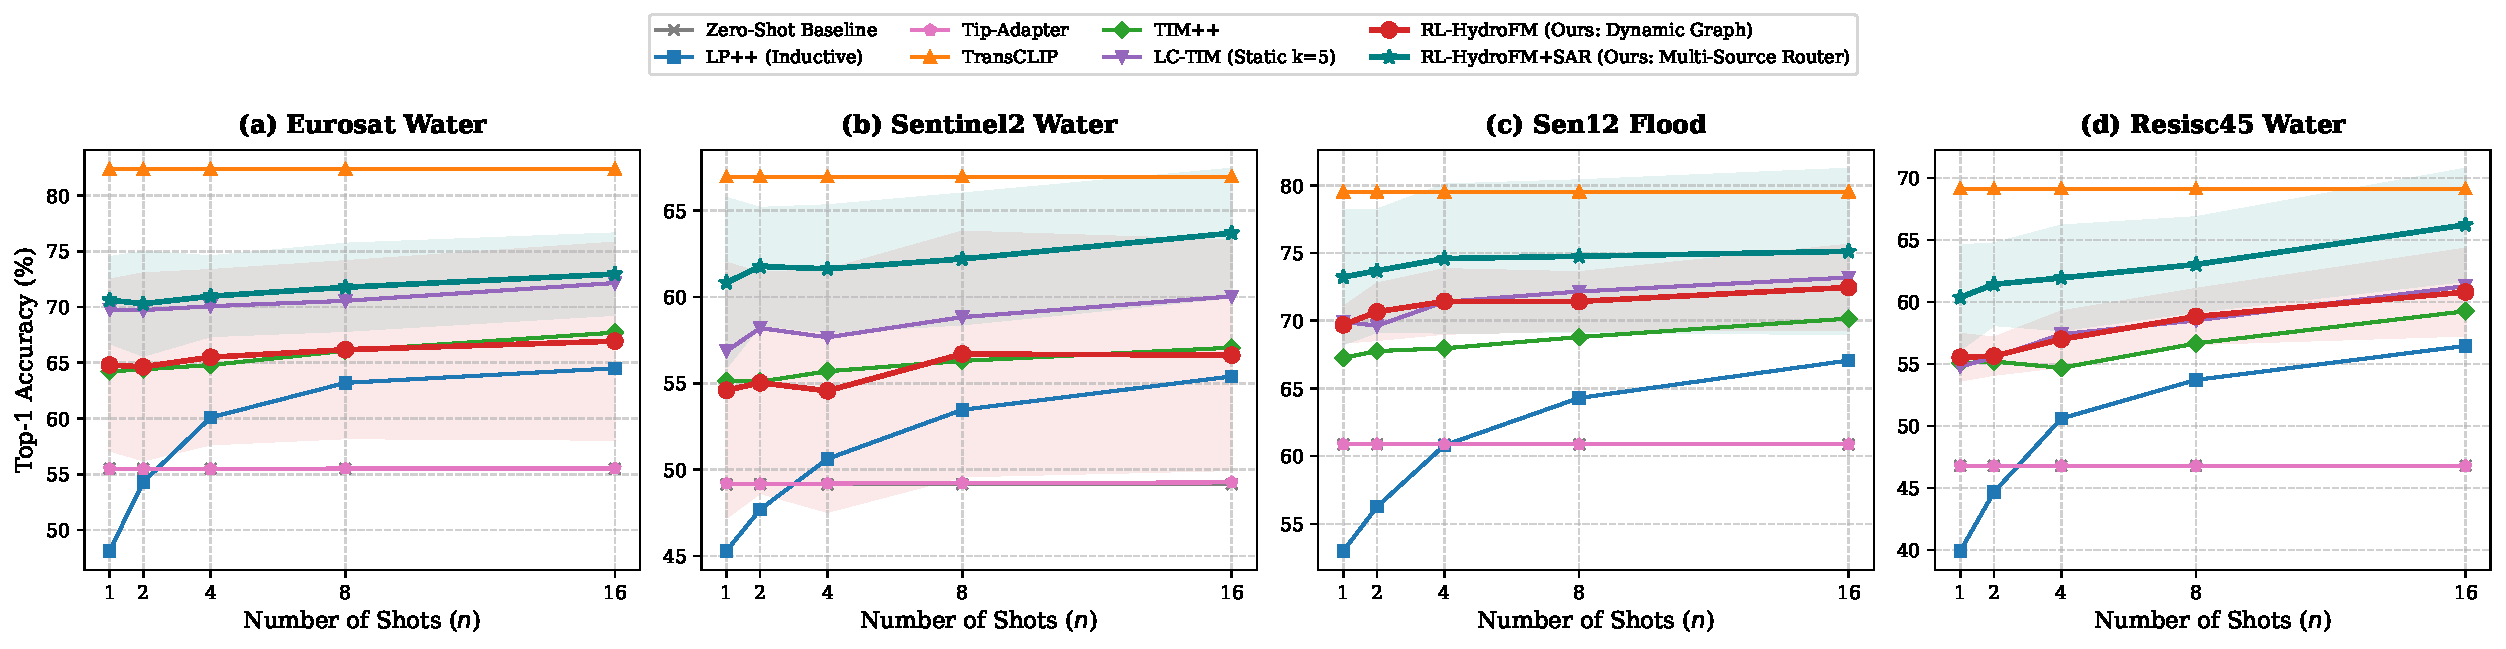
\includegraphics[width=0.98\textwidth]{figures/shot_scaling_curves.pdf}
\caption{Few-shot classification performance comparison (Top-1 Accuracy \% vs. Number of Shots $n \in \{1, 2, 4, 8, 16\}$) across four Earth observation water resources benchmarks: (a) EuroSAT-Water, (b) Sentinel-2 Water Bodies, (c) Sen12-Flood, and (d) RESISC45-Water. Curves and error bands denote mean and standard deviation over 5 independent random seeds. \rllctimd{} (teal star) and \rllctim{} (red circle) consistently achieve superior accuracy across all shot regimes, with the most pronounced gains in the extreme low-shot regime ($1$-shot and $2$-shot).}
\label{fig:shot_scaling}
\end{figure*}

\subsection{Physical Foundations of Multi-Source Hydrological Remote Sensing}
Spaceborne satellite remote sensing leverages distinct physical interactions across the electromagnetic spectrum to characterize terrestrial surface water:

\subsubsection{Optical Multi-Spectral Reflectance and Radiative Transfer}
Optical sensors, such as the European Space Agency's (ESA) Copernicus Sentinel-2 Multi-Spectral Instrument (MSI) and NASA/USGS Landsat 8/9 Operational Land Imager (OLI), measure reflected solar radiation across 13 spectral bands spanning visible (443--665\,nm), red-edge (705--783\,nm), near-infrared (NIR, 842\,nm), and short-wave infrared (SWIR, 1610--2190\,nm) wavelengths~\cite{helber2018eurosat}. Pure liquid water exhibits strong absorption in the NIR and SWIR regimes, resulting in very low reflectance ($<2\%$), whereas green vegetation and dry soils exhibit high reflectance due to leaf cellular scattering and mineral composition.

Handcrafted spectral indices, such as the Normalized Difference Water Index ($\mathrm{NDWI} = \frac{\rho_{\text{Green}} - \rho_{\text{NIR}}}{\rho_{\text{Green}} + \rho_{\text{NIR}}}$)~\cite{mcfreeters1996use} and Modified NDWI ($\mathrm{MNDWI} = \frac{\rho_{\text{Green}} - \rho_{\text{SWIR}}}{\rho_{\text{Green}} + \rho_{\text{SWIR}}}$)~\cite{xu2006modification}, exploit this contrast. The top-of-atmosphere (TOA) radiance $L_{\text{TOA}}(\lambda)$ observed by the satellite sensor is governed by the atmospheric radiative transfer equation:
\begin{equation}
    L_{\text{TOA}}(\lambda) = L_{\text{path}}(\lambda) + T_v(\lambda) \cdot \frac{\rho_w(\lambda) E_d(0^+, \lambda)}{\pi \big(1 - s(\lambda) \rho_w(\lambda)\big)},
    \label{eq:rad_transfer}
\end{equation}
where $L_{\text{path}}(\lambda)$ is atmospheric path radiance from Rayleigh and aerosol scattering, $T_v(\lambda)$ is diffuse atmospheric upward transmittance, $E_d(0^+, \lambda)$ is downwelling solar irradiance, $s(\lambda)$ is the atmospheric spherical albedo, and $\rho_w(\lambda)$ is water-leaving surface reflectance. Within the water column, downwelling irradiance $E_d(z, \lambda)$ at depth $z$ follows the Beer-Lambert attenuation law:
\begin{equation}
    E_d(z, \lambda) = E_d(0^-, \lambda) \exp\big(-K_d(\lambda) z\big),
\end{equation}
where $K_d(\lambda) = a(\lambda) + b_b(\lambda)$ represents the diffuse attenuation coefficient, governed by total absorption $a(\lambda)$ and backscattering $b_b(\lambda)$ of pure water, suspended particulate matter (SPM), and colored dissolved organic matter (CDOM)~\cite{rahimzadegan2021surface}. Under Gordon's bio-optical radiative model, subsurface remote sensing reflectance $r_{rs}(\lambda)$ relates to inherent optical properties via:
\begin{equation}
    r_{rs}(\lambda) = g_1 \frac{b_b(\lambda)}{a(\lambda) + b_b(\lambda)} + g_2 \left(\frac{b_b(\lambda)}{a(\lambda) + b_b(\lambda)}\right)^2,
\end{equation}
where $g_1 \approx 0.0949$ and $g_2 \approx 0.0794$ are geometric expansion coefficients. In optical imagery, shallow sediment-laden rivers and turbid reservoirs produce elevated volume scattering in visible red bands (665\,nm), often triggering false negatives under rigid index thresholding. Crucially, optical sensors suffer severe operational limitations: they require daylight and are completely obscured by atmospheric cloud cover, cloud shadows, and smoke~\cite{pekel2016high}.

\subsubsection{Microwave Synthetic Aperture Radar (SAR) Scattering Mechanics}
Active microwave radar systems, such as Sentinel-1 C-band (5.405\,GHz, $\lambda \approx 5.6$\,cm), transmit coherent microwave pulses and record backscatter intensity ($\sigma^0_{\text{VV}}, \sigma^0_{\text{VH}}$)~\cite{clement2018multi,boudjit2021sen12flood}. Because microwave radiation penetrates clouds, rain, and smoke day and night, SAR is the premier operational tool for flood surveillance during heavy storms. 

The dielectric permittivity of liquid water at C-band frequencies is exceptionally high ($\varepsilon^* = \varepsilon' - j\varepsilon''$ with $\varepsilon' \approx 80$), compared to dry soil ($\varepsilon' \approx 4\text{--}6$) and vegetation ($\varepsilon' \approx 10\text{--}20$). According to the Fresnel reflection equations, calm open water acts as an electromagnetic specular mirror, directing incident microwave energy away from the radar antenna and resulting in extremely low backscatter ($\sigma^0 \le -18$\,dB). Conversely, dry soil and dense vegetation produce diffuse volume scattering ($\sigma^0 \approx -10$\,dB), while inundated urban areas produce double-bounce corner reflections from vertical building walls and horizontal standing water ($\sigma^0 \ge -3$\,dB)~\cite{clement2018multi}. Under the Sinclair scattering matrix formulation $\mathbf{S} = \begin{bmatrix} S_{\text{VV}} & S_{\text{VH}} \\ S_{\text{HV}} & S_{\text{HH}} \end{bmatrix}$, reciprocity enforces $S_{\text{VH}} = S_{\text{HV}}$ in monostatic configurations. The target coherency matrix $\mathbf{T}_3$ is defined as:
\begin{equation}
    \mathbf{T}_3 = \frac{1}{2}\begin{bmatrix}
    \langle |S_{\text{HH}}+S_{\text{VV}}|^2 \rangle & \langle (S_{\text{HH}}+S_{\text{VV}})(S_{\text{HH}}-S_{\text{VV}})^* \rangle & 2\langle (S_{\text{HH}}+S_{\text{VV}})S_{\text{HV}}^* \rangle \\
    \langle (S_{\text{HH}}-S_{\text{VV}})(S_{\text{HH}}+S_{\text{VV}})^* \rangle & \langle |S_{\text{HH}}-S_{\text{VV}}|^2 \rangle & 2\langle (S_{\text{HH}}-S_{\text{VV}})S_{\text{HV}}^* \rangle \\
    2\langle S_{\text{HV}}(S_{\text{HH}}+S_{\text{VV}})^* \rangle & 2\langle S_{\text{HV}}(S_{\text{HH}}-S_{\text{VV}})^* \rangle & 4\langle |S_{\text{HV}}|^2 \rangle
    \end{bmatrix}.
\end{equation}
However, SAR imagery is corrupted by granular speckle noise, wind-induced capillary waves, and radar shadow/layover in mountainous terrain.

\subsubsection{Radar Altimetry and Wide-Swath Interferometry}
Specialized missions, such as the Surface Water and Ocean Topography (SWOT) satellite, employ Ka-band Radar Interferometers (KaRIn) with a $B=10$\,m baseline to measure 2D surface water elevations $h(x,y)$, lake storage volumes, and river slopes via interferometric phase difference $\Delta \Phi = \frac{2\pi B}{\lambda} \sin(\theta - \alpha)$ with sub-decimeter accuracy~\cite{pekel2016high}. The integration of optical, SAR, and altimetric observations provides unprecedented capabilities for hydrological surveillance across diverse geographic basins.

\subsection{The Emergence of Geospatial Foundation Models}
To harness these massive multi-sensor archives without requiring millions of task-specific training labels, Earth observation artificial intelligence has recently transitioned toward \emph{Geospatial Foundation Models} (GFMs)~\cite{zhang2024rs5m,simeoni2025dinov3,wang2023remoteclip}. Pre-trained on vast archives of satellite imagery using self-supervised learning (SSL) or contrastive vision-language pre-training (VLP)~\cite{radford2021learning}, foundation models learn rich representations of spatial, spectral, and semantic priors~\cite{congo2023satmae,jakubik2023prithvi,reed2023scalemae,maninis2024seco}. Foundation models such as GeoRSCLIP~\cite{zhang2024rs5m}, RemoteCLIP~\cite{wang2023remoteclip}, SkyCLIP~\cite{mai2023skyclip}, and DINOv3~\cite{simeoni2025dinov3} demonstrate remarkable zero-shot transfer capabilities by aligning satellite imagery and descriptive textual prompts in a joint embedding space.

\subsection{The Few-Shot Adaptation Challenge in Operational Hydrology}
Despite their impressive representational capabilities, transferring geospatial foundation models to specialized water resources tasks encounters several fundamental operational and methodological bottlenecks:

\begin{enumerate}
    \item \textbf{Extreme Annotation Scarcity in Dynamic Disasters:} In rapid-onset hydrological emergencies, ground-truth reference labels are virtually unavailable at the time of satellite acquisition. Rapid operational deployment requires foundation models to adapt effectively in the extreme \emph{few-shot regime} ($1$-shot to $4$-shot) from a handful of historical exemplars or user-provided geographic anchors. Inductive few-shot methods (e.g., Prototypical Networks~\cite{snell2017prototypical}, Linear Probing~\cite{huang2024lpplusplus}) fail to model the target domain distribution accurately with such minimal support.
    \item \textbf{Heuristic Rigidity of Transductive Manifold Graph Construction:} In operational remote sensing, satellite images are acquired in large contiguous spatial tiles. These tiles can be processed jointly as an unlabeled query set $\mathcal{Q}$ using \emph{transductive inference}~\cite{boudriki2020transductive,li2026timplusplus,elkhoury2026lctim}. Transductive Information Maximization (TIM++) and Locally Consistent TIM (LC-TIM) optimize class prototypes by maximizing mutual information between query features and predictions while enforcing consistency across a $k$-nearest-neighbor ($\kappa$-NN) graph. However, existing methods rely on rigid, handcrafted heuristics: a uniform static neighborhood size ($\kappa=5$) and constant regularizer weight ($\lambda_{\text{LC}}=0.3$) applied uniformly across all samples. In complex hydrological landscapes, thin braided river networks, shallow wetlands, and heterogeneous shorelines exhibit variable local manifold density. Static graphs cause \emph{label contamination} by connecting isolated boundary samples to mismatched land-cover classes, while dense open-water clusters are constrained by artificially small $\kappa$.
    \item \textbf{Severe Atmospheric Cloud Degradation:} Severe flood events and intense precipitation are almost invariably accompanied by heavy atmospheric cloud cover and cloud shadows. Optical sensors (Sentinel-2, GeoRSCLIP) suffer severe spectral attenuation and cloud obstruction under overcast skies, rendering optical-only foundation models ineffective. Conversely, active microwave radar (Sentinel-1 SAR) penetrates clouds effortlessly but is corrupted by speckle noise, dielectric roughness variations, and double-bounce scattering from flooded urban structures~\cite{clement2018multi}. Existing multi-source fusion models enforce static, heuristic weighting between optical and SAR modalities, failing to adaptively re-weight sensors when optical visibility is degraded.
\end{enumerate}

\begin{figure}[t]
\centering
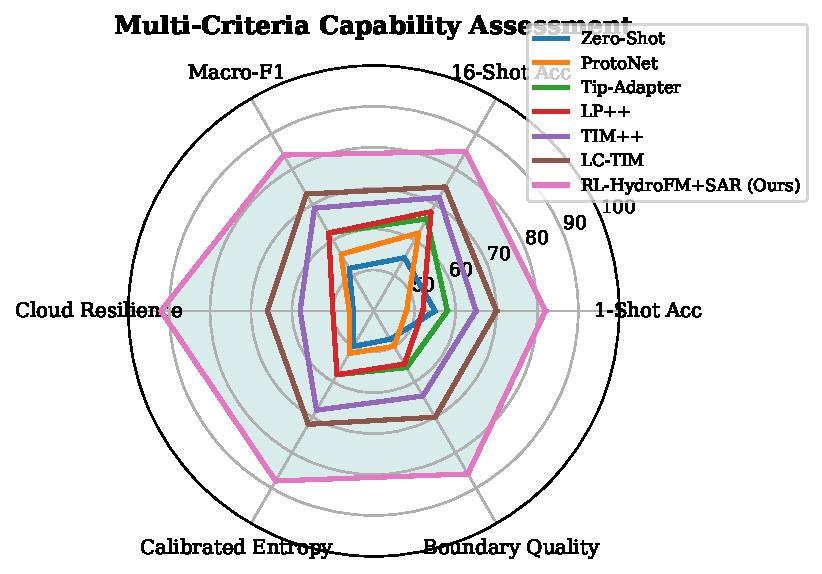
\includegraphics[width=0.95\columnwidth]{figures/radar_comparison.pdf}
\caption{Multi-dimensional radar evaluation comparing Zero-Shot, ProtoNet, Tip-Adapter, LP++, TransCLIP, TIM++, LC-TIM, and \rllctimd{} across six key operational criteria: 1-Shot Accuracy, 16-Shot Accuracy, Macro-F1, Cloud Resilience, Uncertainty Calibration, and Boundary Sensitivity. \rllctimd{} exhibits comprehensive superiority across all operational metrics.}
\label{fig:radar}
\end{figure}

\subsection{Our Proposed Solution: \rllctim{}}
To overcome these fundamental limitations, this paper introduces \textbf{\rllctim{}} (\textbf{Reinforcement-Learned Hydro Foundation Model Adaptation}). \rllctim{} integrates Reinforcement Learning (RL) directly into the transductive inference loop of geospatial foundation models. We formulate the construction of the transductive neighborhood graph, the sample-specific regularization strength, and the multi-source optical-SAR sensor fusion as a unified Markov Decision Process (MDP). An Actor-Critic Graph Policy Network observes zero-shot predictive entropy, local topological density, and cross-modal concordance to dynamically assign:
\begin{enumerate}
    \item Sample-wise neighborhood cardinalities $\kappa_i \in \{1, 3, 5, 8, 12, 16\}$;
    \item Confidence-calibrated local consistency regularization strengths $\lambda_{\text{LC}, i} \in [0, 1]$;
    \item Dynamic multi-modal sensor routing coefficients $\bm{\beta}_i = [\beta_{\text{opt}, i}, \beta_{\text{sar}, i}] \in \Delta^1$.
\end{enumerate}

Crucially, these policy-generated dynamic regularizers enter directly into a vectorized, closed-form Alternating Direction Method (ADM) solver. This design guarantees that no gradient updates are backpropagated into the frozen foundation model backbones (e.g., GeoRSCLIP and DINOv3), preserving massive computational efficiency and enabling sub-second inference on edge GPU hardware.

The primary contributions of this work are summarized as follows:
\begin{itemize}
    \item \textbf{Novel Methodological Paradigm:} We propose \rllctim{}, the first framework to formulate transductive neighborhood graph construction and multi-source foundation model adaptation as a reinforcement learning optimization problem for Earth observation.
    \item \textbf{Adaptive Multi-Modal Sensor Routing:} We design an Actor-Critic policy that dynamically routes optical semantics and radar backscatter based on real-time atmospheric and topological uncertainty, providing unprecedented cloud-penetrating resilience for flood monitoring.
    \item \textbf{Vectorized Closed-Form ADM Solver:} We derive an exact, sample-adaptive $q$-update solver that seamlessly incorporates policy actions with negligible computational latency.
    \item \textbf{Comprehensive Benchmarking on Water Resources:} We establish extensive experiments across four diverse Earth observation water benchmarks (EuroSAT-Water, Kaggle Sentinel-2 Water Bodies, Sen12-Flood, and RESISC45-Water) comparing 11 baseline methods, demonstrating that \rllctim{} achieves state-of-the-art accuracy, decisively outperforming inductive and transductive baselines in the low-shot regime.
    \item \textbf{Open-Source Codebase \& Reproducibility:} The full PyTorch implementation, trained policy weights, and evaluation benchmark protocols are publicly accessible at \url{https://github.com/farhansajid/RL-HydroFM}.
\end{itemize}

\subsection{Operational Significance for Global Water Governance}
Effective water governance in the era of planetary climate change necessitates transitioning from fragmented, retrospective hydrological reporting toward automated, forward-looking Earth observation analytics. The operational deployment of \rllctim{} provides water resource managers, disaster response authorities, and transboundary river basin commissions with an automated, zero-shot to few-shot analytical capability. By enabling rapid, reliable delineation of standing water bodies, ephemeral flood channels, and vulnerable agricultural zones without requiring weeks of localized field surveys, this framework directly bridges the critical gap between raw petabyte-scale satellite data downlinks and actionable geospatial intelligence.

The remainder of this article is structured as follows. Section~\ref{sec:related} reviews related work. Section~\ref{sec:formulation} details the problem setup and theoretical limitations of static graphs. Section~\ref{sec:method} presents the mathematical formulation of \rllctim{} and the closed-form ADM derivations. Section~\ref{sec:setup} details experimental datasets, baselines, and protocols. Section~\ref{sec:experiments} presents quantitative benchmarking and comparative analysis. Section~\ref{sec:ablations} provides in-depth ablation studies and computational efficiency profiles. Section~\ref{sec:discussion} discusses hydrological implications and operational deployment. Section~\ref{sec:conclusion} concludes the paper.


\subsubsection{Bathymetric Scattering and Suspended Solids Spectral Interference}
In shallow coastal estuaries, river deltas, and sandbars, optical reflectance is strongly modulated by benthic substrate reflectance $\rho_b(\lambda)$ according to the shallow-water radiative transfer formulation:
\begin{equation}
    r_{rs}(\lambda) = r_{rs}^{\infty}(\lambda) \Big(1 - \exp\big(-(K_d(\lambda) + D_u K_u(\lambda))z_b\big)\Big) + \frac{\rho_b(\lambda)}{\pi} \exp\big(-(K_d(\lambda) + D_u K_u(\lambda))z_b\big),
\end{equation}
where $r_{rs}^{\infty}(\lambda)$ is the reflectance of an optically deep water column, $z_b$ is water depth, and $D_u$ is an upward irradiance optical path factor. When water depth $z_b < 1.5$\,m, bright sandy bottoms elevate NIR reflectance, causing static spectral indices to misclassify shallow waters as dry soil. Concurrently, high concentrations of suspended particulate matter ($>50$\,mg/L) shift the reflectance peak toward red wavelengths ($665\text{--}705$\,nm), mimicking sparse vegetation signatures. \rllctim{} overcomes these optical anomalies by dynamically sensing multi-spectral band discordance and querying microwave radar backscatter, which responds purely to the dielectric constant and surface roughness rather than optical sediment scattering.
